\documentclass{beamer}

\mode<presentation> {

\usetheme{Copenhagen}
\usecolortheme{seagull}
}

\usepackage{graphicx}
\DeclareGraphicsExtensions{.pdf,.png,.jpg}
\usepackage{booktabs} % Allows the use of \toprule, \midrule and \bottomrule in tables
\usepackage{mathtools}
\usepackage{multirow}
\usepackage{color, colortbl}
\usepackage{minted}

%----------------------------------------------------------------------------------------
%	TITLE PAGE
%----------------------------------------------------------------------------------------

\title[Test]{Test}

\author{Rasmus Guldborg Pedersen}

\date{June 2015}

\begin{document}

\begin{frame}
\titlepage
\end{frame}

\begin{frame}
\frametitle{Overview}
\tableofcontents
\end{frame}



\section{Q 2.9: Agile testing}

\begin{frame}
    \frametitle{Traditional vs Agile}
    \begin{columns}[c]
        \column{0.5\textwidth}
        \begin{block}{Traditional Testing}
            \begin{itemize}
                \item Separate team
                \item Separate process
                \item Tension between developers and testers
                    % Developers spit out code, throw it over the wall to
                    % testers
                    % Testers detect defects throw it over the wall to
                    % developers
            \end{itemize}
        \end{block}

        \column{0.5\textwidth}
        \begin{block}{Agile Testing}
            \begin{itemize}
                \item Testers are part of the development team
                \item Testing is part of the development process
                \item Shared goal
                    % Both testers and developers share the same goal of
                    % fulfilling user stories.
            \end{itemize}
        \end{block}
    \end{columns}
\end{frame}

\begin{frame}
    \frametitle{Agile Testing Quadrants}
    \centering
    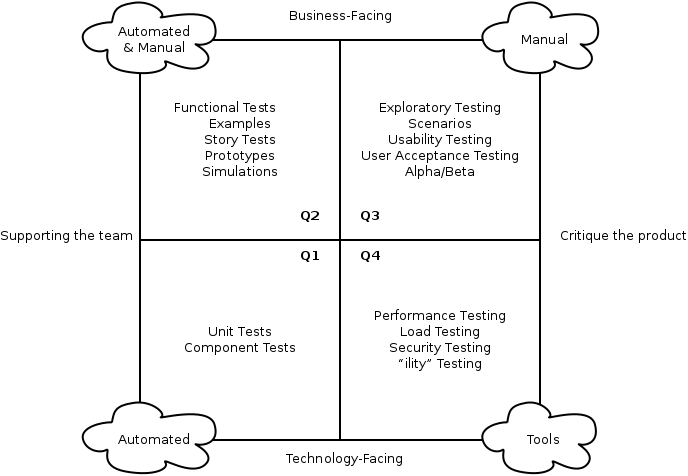
\includegraphics[scale=0.4]{agile_test_quadrants.png}
\end{frame}

\begin{frame}
    \frametitle{Test Driven Development}
    \begin{columns}
        \column{0.5\textwidth}
        \begin{itemize}
            \item Red-green testing
            \item All code has tests
            \item Closing the feedback loop
        \end{itemize}

        \column{0.5\textwidth}
        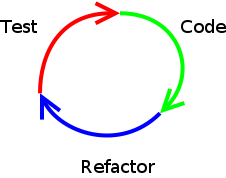
\includegraphics[scale=0.5]{tdd_cycle.png}
    \end{columns}
\end{frame}

\begin{frame}
    \frametitle{Continuous Integration}
    \begin{itemize}
        \item Integrate often
        \item Integration becomes cheap
        \item Automate build
        \item Test on build
    \end{itemize}
\end{frame}


%------------------------------------------------

\begin{frame}
    \frametitle{The End}

    %\Huge{\centerline{The End}}
    \begin{quote}
        ``Testing shows the presence, not the absence of bugs.''
        \raggedleft{--- Edsger W. Dijkstra}
    \end{quote}
\end{frame}

%----------------------------------------------------------------------------------------

\end{document}

